\documentclass[12pt,a4paper]{article}
\usepackage[T1]{fontenc}
\usepackage[utf8]{inputenc}
\usepackage[provide=*,turkish]{babel}
\usepackage{mathptmx}
\usepackage[a4paper,margin=2.5cm,headheight=16pt]{geometry}
\usepackage{graphicx,caption,booktabs,tabularx,enumitem}
\usepackage{tikz}
\usetikzlibrary{arrows.meta,positioning,shapes.geometric}
\usepackage{xcolor}
\definecolor{baslik}{HTML}{17365D}
\usepackage{titlesec}
\titleformat{\section}{\Large\bfseries\color{baslik}}{\thesection}{.7em}{}
\titleformat{\subsection}{\large\bfseries\color{baslik}}{\thesubsection}{.7em}{}
\usepackage{fancyhdr,lastpage}
\pagestyle{fancy}\fancyhf{}


\newcommand{\ogrenciad}{Ad Soyad}
\newcommand{\ogrencino}{Öğrenci numarası}

\fancyhead[L]{\small \ogrenciad\enspace--\enspace\ogrencino}
\fancyhead[R]{\small EHB326E}

\fancyfoot[C]{\thepage\ / \pageref{LastPage}}
\renewcommand{\headrulewidth}{0.4pt}
\usepackage{ragged2e}
\AtBeginDocument{\justifying}
\usepackage{hyperref}
\hypersetup{colorlinks=true,linkcolor=baslik,urlcolor=baslik,citecolor=baslik}

\newcommand{\raporbasligi}{Ödev Başlığı}

\begin{document}
\begin{center}
{\Large\bfseries İstanbul Teknik Üniversitesi}\\[5pt]
{\large EHB326E -- Ödev N Raporu}\\[18pt]
{\LARGE\bfseries\color{baslik}\raporbasligi}\\[15pt]
\ogrenciad\quad(\ogrencino)\\[5pt]
\today
\end{center}
\vspace{1em}
\section{Özet}
Bu bölümde tasarımın amacı, kullanılan yöntem ve doğrulanan sonuçlar kısa biçimde açıklanır. Ölçülmemiş başarı veya performans değerleri yazılmamalıdır.

\section{Amaç ve Gereksinimler}
Ödevin hedefini ve gereksinimlerini yazınız.

\section{Yöntem ve Sistem Tasarımı}
Gerekliyse sistemin bileşenlerini ve veri akışını açıklayınız. Aşağıdaki diyagramı kendi tasarımınıza göre düzenleyiniz.

\begin{figure}[htbp]\centering
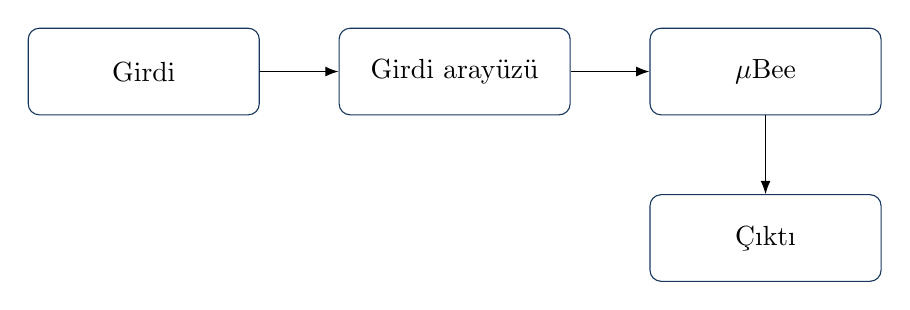
\begin{tikzpicture}[node distance=10mm and 10mm, >=Latex,
 block/.style={draw=baslik,rounded corners,align=center,minimum height=11mm,text width=27mm}]
\node[block] (girdi) {Girdi};
\node[block,right=of girdi] (arayuz) {Girdi arayüzü};
\node[block,right=of arayuz] (sistem) {$\mu$Bee};
\node[block,below=of sistem] (cikti) {Çıktı};
\draw[->] (girdi)--(arayuz);\draw[->] (arayuz)--(sistem);\draw[->] (sistem)--(cikti);
\end{tikzpicture}
\caption{Örnek sistem akışı; gerçek uygulamaya göre güncellenmelidir.}
\label{fig:akis}
\end{figure}

\subsection{Gerçekleme}
Kodu rapora yapıştırmayınız. Önemli modüllerin görevi, giriş ve çıkışları, zamanlaması ve tasarım tercihleri anlatılır; kaynak dosyalar teslim paketinde ayrı tutulur.

\section{Simülasyon ve Bulgular}
Test koşullarını, uygulanan girişleri (Kod verilmeyecek), beklenen davranışı ve gözlenen çıktıyı veriniz. Her şekle metinde atıf yapınız; sonuçları yorumlayınız.
\begin{table}[htbp]\centering
\caption{Test ve gözlem kayıtları}\label{tab:test}
\begin{tabularx}{\linewidth}{@{}lXXX@{}}\toprule
Test & Giriş / koşul & Beklenen sonuç & Gözlenen sonuç \\ \midrule
1 & [Doldurunuz] & [Doldurunuz] & [Doldurunuz] \\
2 & [Doldurunuz] & [Doldurunuz] & [Doldurunuz] \\ \bottomrule
\end{tabularx}
\end{table}

% Ekran görüntüsünü Images/ dizinine koyun. Kırpmayı trim={sol alt sağ üst},clip ile ayarlayın.
% \begin{figure}[htbp]\centering
% \includegraphics[width=.9\linewidth,trim={12mm 8mm 12mm 8mm},clip]{Images/simulasyon.png}
% \caption{Simülasyon sonucu ve ilgili test koşulu.}\label{fig:simulasyon}
% \end{figure}

\section{Doğrulama ve Değerlendirme}
Tasarımın doğru çalışıp çalışmadığını, beklenen sonuçların hangilerinin elde edildiğini ve varsa sınırlamaları açıkça yazınız. Tablo~\ref{tab:test} ile değerlendirmenizi destekleyiniz.

\section{Sonuç}
Ulaşılan sonuçları ve tasarımın hedefleri karşılama durumunu kısaca özetleyiniz.

\begin{thebibliography}{99}
% Kullanılan kaynakları burada sırasıyla numaralandırın; metinde \cite{ornek} kullanın.
% \bibitem{ornek} Yazar/Kurum, \emph{Eser veya sayfa başlığı}, yıl, \url{https://...}, erişim: GG.AA.YYYY.
\end{thebibliography}
\end{document}
